\section{System Model}
\label{sec:model}
The proposed ATEF-DT is an adaptive trust-aware and energy-fair framework for scheduling battery-constrained clients in federated digital-twin healthcare. As shown in Fig.~\ref{fig:architecture}, each training round passes through four modules. The patient-centric digital twin (A) tracks the patient's state from noisy sensor readings and forecasts the monitoring energy the device must reserve. The energy-aware client selection module (B) assigns each client a bit-width, removes clients whose round energy would breach this reserve, and ranks the rest by a weighted-product score over energy, participation and reputation. The local training and adaptive quantization module (C) trains each selected client and uploads its update at the assigned bit-width. Finally, the credibility-based aggregation module (D) scores each update against a geometric-median reference, updates the reputations, and aggregates the clipped, accepted updates with reputation weights.

Formally, a server coordinates the clients $\cP=\{1,\dots,P\}$ over $R$ rounds and selects at most $S_{\max}$ of them per round. Client $p$ is the edge node of one patient; it holds a local data set $\mathcal{D}_p$ of $N_p$ samples ($N=\sum_{p}N_p$), a battery with residual energy $C_p^{(r)}$ and the patient's digital twin. Table~\ref{tab:notation} lists the notation.

\rtag{E1, R1.1, R2.1}\begin{revblock}Each module builds on an established component, namely Kalman state tracking~\cite{kalman1960new}, wireless-FL energy models~\cite{tran2019federated,yang2021energy}, product scalarization~\cite{marler2004survey}, stochastic quantization~\cite{alistarh2017qsgd} and robust aggregation~\cite{pillutla2022robust,cao2021fltrust,karimireddy2021learning}. The contribution lies in their coupling: the twin forecast decides whether a device may train, one scale-invariant score combines the three criteria, the bit-width adapts to each device, and aggregation uses reputation weights instead of client-reported sizes.\end{revblock}

\begin{figure*}[t]
	\centering
	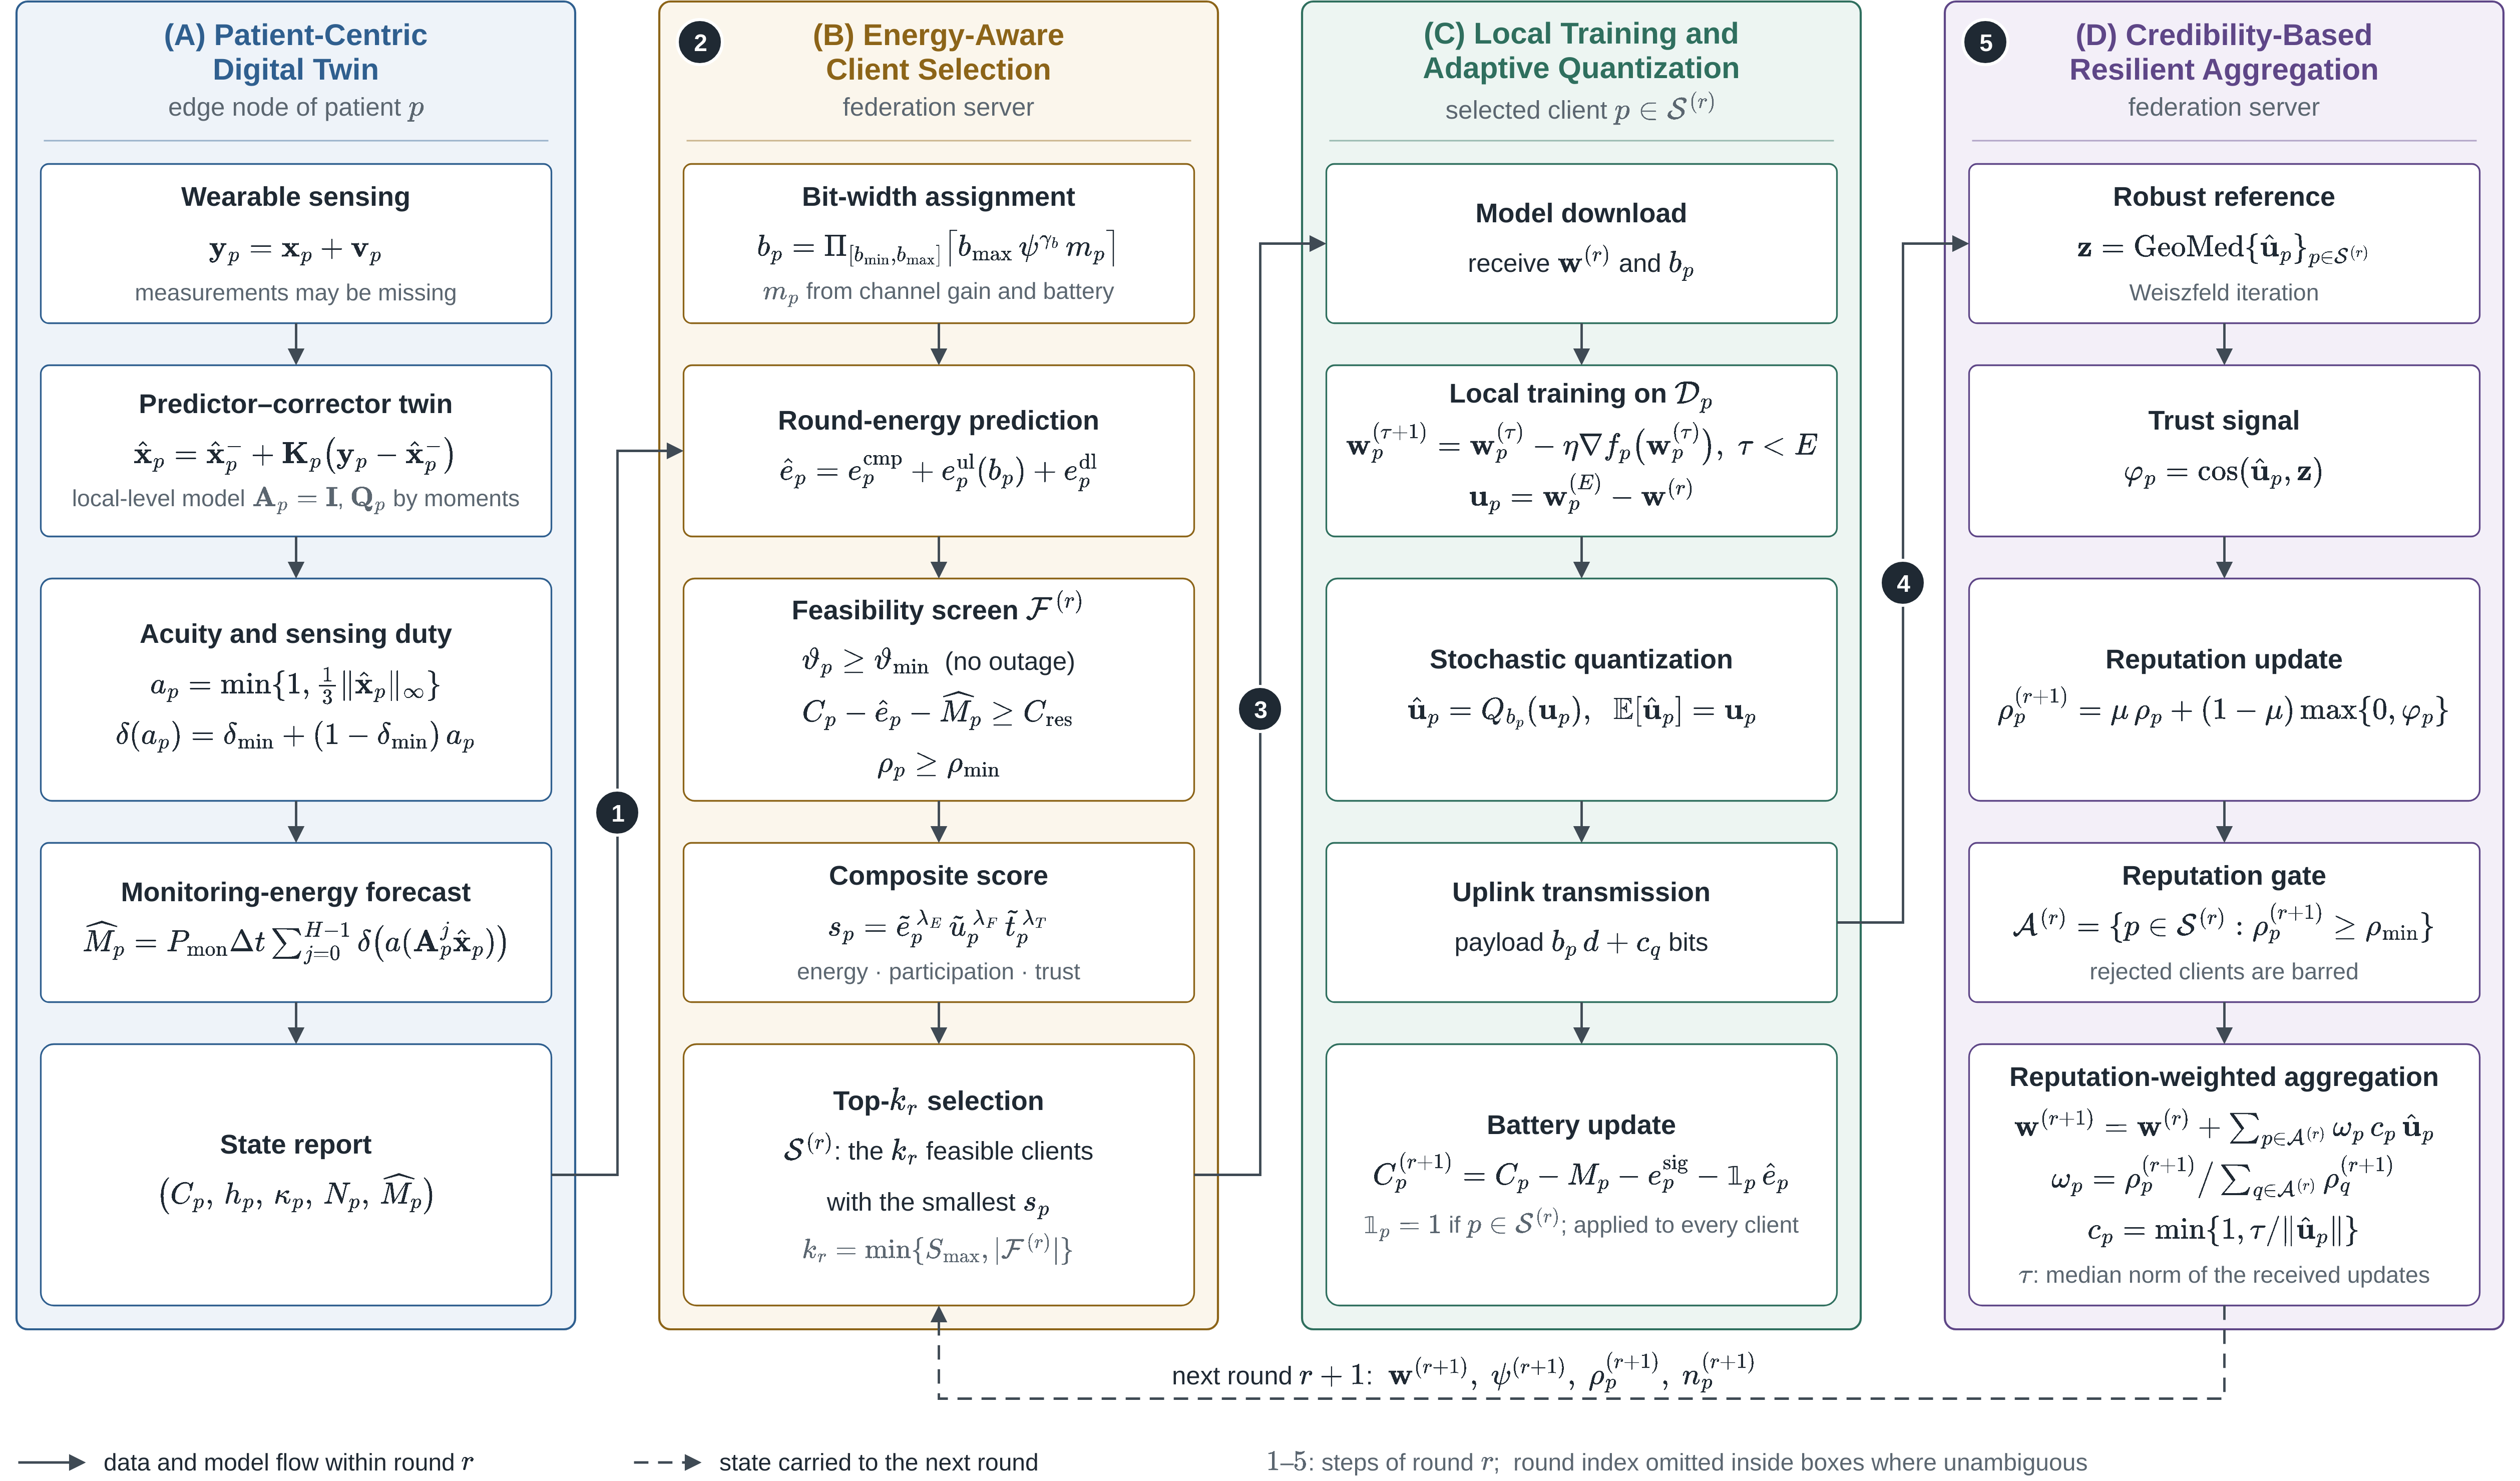
\includegraphics[width=\textwidth]{figures/fig_framework.png}
	\revcap{E6, R1.7(6), R2.6}{Architecture of ATEF-DT: (A)~patient-centric digital twin, (B)~energy-aware client selection, (C)~local training and adaptive quantization, and (D)~credibility-based resilient aggregation. Numbers 1--5 mark the steps of a round; the dashed arrow carries the state to the next round.}
	\label{fig:architecture}
\end{figure*}

\begin{table}[t]
	\centering
	\revcap{R1.7(8)}{Notation.}
	\label{tab:notation}
	\footnotesize
	\setlength{\tabcolsep}{3pt}
	\begin{tabularx}{\columnwidth}{l >{\raggedright\arraybackslash}X}
		\toprule
		\textbf{Symbol} & \textbf{Meaning} \\
		\midrule
		$\cP$, $P$ & set and number of clients \\
		$R$, $S_{\max}$ & number of rounds; per-round selection budget \\
		$\mathcal{D}_p$, $N_p$, $N$ & local data set, its size, total number of samples \\
		$\w^{(r)}\in\mathbb{R}^d$ & global model at round $r$ \\
		$\uu_p^{(r)}$, $\uh_p^{(r)}$ & local update of client $p$; quantized update received by the server \\
		$\eta$, $E$ & learning rate; number of local passes \\
		$\cF^{(r)}$, $\cS^{(r)}$, $\cA^{(r)}$ & feasible, selected and accepted sets \\
		$C_p^{(r)}$, $C_{\mathrm{res}}$ & residual battery energy; reserve \\
		$\kappa_p$, $h_p^{(r)}$, $\vartheta_p^{(r)}$ & computation factor; channel power gain; uplink spectral efficiency \\
		$\hat e_p^{(r)}$ & predicted energy of the round for client $p$ \\
		$\hat{\x}_p^{(r)}$, $a_p^{(r)}$, $\delta(\cdot)$ & twin state estimate; acuity; sensing duty \\
		$M_p^{(r)}$, $\widehat{M}_p^{(r)}$ & monitoring energy of a round; its forecast over $H$ rounds \\
		$b_p^{(r)}$, $\psi^{(r)}$ & bit-width; stability surrogate \\
		$\z^{(r)}$, $\varphi_p^{(r)}$ & geometric-median reference; cosine trust signal \\
		$\rho_p^{(r)}$, $\mu$, $\rho_{\min}$ & reputation; forgetting factor; threshold \\
		$c_p^{(r)}$, $\omega_p^{(r)}$, $\beta_p^{(r)}$ & clipping factor; reputation weight; coefficient $\omega_p c_p$ \\
		$n_p^{(r)}$ & number of rounds before $r$ in which $p$ was selected \\
		$\tilde e_p,\tilde u_p,\tilde t_p$ & energy, participation and trust factors \\
		$\lambda_E,\lambda_F,\lambda_T$ & exponents of the score \\
		\bottomrule
	\end{tabularx}
\end{table}

\subsection{Problem Formulation}
\label{subsec:problem}
The learning objective is the empirical risk over all clients,
\begin{equation}
	F(\w)=\sum_{p\in\cP}\frac{N_p}{N}\,f_p(\w),\qquad f_p(\w)=\frac{1}{N_p}\sum_{(\x,y)\in\mathcal{D}_p}\ell(\w;\x,y),
	\label{eq:objective}
\end{equation}
where $\ell$ is the loss of one sample; this is the standard federated objective, in which each client counts in proportion to its data~\cite{mcmahan2017communication,kairouz2021advances}. The scheduler chooses, in every round, the selected set $\cS^{(r)}$ and the bit-widths $b_p^{(r)}$. Three quantities describe the cost of a schedule over the horizon: the device energy, the disparity of participation and the exposure to updates of low credibility,
\begin{equation}
	\begin{aligned}
		E_{\mathrm{tot}}&=\sum_{r=0}^{R-1}\sum_{p\in\cS^{(r)}}\hat e_p^{(r)}, \qquad D_{\mathrm{part}}=1-J\bigl(\mathbf{n}^{(R)}\bigr),\\
		T_{\mathrm{exp}}&=\sum_{r=0}^{R-1}\sum_{p\in\cS^{(r)}}\bigl(1-\rho_p^{(r)}\bigr),
	\end{aligned}
	\label{eq:criteria}
\end{equation}
where $J(\mathbf{n})=(\sum_p n_p)^2/(P\sum_p n_p^2)$ is the Jain index~\cite{jain1984quantitative} of the participation counts. The index equals one when all clients have taken part equally often and $1/P$ when a single client has taken part every time, so $D_{\mathrm{part}}$ grows as participation concentrates on a few clients. The design problem is the multi-objective program
\begin{equation}
	\begin{aligned}
		\min_{\{\cS^{(r)},\,b^{(r)}\}}\quad & \bigl(F(\w^{(R)}),\;E_{\mathrm{tot}},\;D_{\mathrm{part}},\;T_{\mathrm{exp}}\bigr)\\
		\text{s.t.}\quad & |\cS^{(r)}|\le S_{\max},\quad b_{\min}\le b_p^{(r)}\le b_{\max},\\
		& C_p^{(r)}-\hat e_p^{(r)}-\widehat{M}_p^{(r)}\ge C_{\mathrm{res}}\quad\text{for all } p\in\cS^{(r)} \text{ and all } r .
	\end{aligned}
	\label{eq:designproblem}
\end{equation}
The last constraint protects the clinical function of the device: a client may train only if, after paying for the round, it keeps enough energy to monitor its patient over the next $H$ rounds, with the forecast $\widehat{M}_p^{(r)}$ defined in Section~\ref{subsec:twin}.

\rtag{E2, R1.2, R2.2}\begin{revblock}Problem~\eqref{eq:designproblem} cannot be solved online. The final loss depends on updates that have not yet been computed, the channel gains are revealed one round at a time, and the reputations are produced by the procedure itself. ATEF-DT therefore does not solve~\eqref{eq:designproblem}. It applies a myopic rule in each round, and the rule is a heuristic. What the rule optimizes is the per-round surrogate
\begin{equation}
	\min_{\cS\subseteq\cF^{(r)},\;|\cS|=k_r}\;\sum_{p\in\cS}\bigl(\lambda_E\ln\tilde e_p+\lambda_F\ln\tilde u_p+\lambda_T\ln\tilde t_p\bigr),
	\label{eq:roundproblem}
\end{equation}
with $k_r=\min\{S_{\max},|\cF^{(r)}|\}$, where $\cF^{(r)}$ is the feasible set and $\tilde e_p,\tilde u_p,\tilde t_p>0$ are per-round criteria defined in Section~\ref{subsec:score}. Problem~\eqref{eq:roundproblem} is a weighted-product scalarization~\cite{marler2004survey} of the three per-round criteria. It is not the Lagrangian of~\eqref{eq:designproblem}, and its exponents are preference weights, not multipliers: a Lagrangian relaxation of additive long-run costs leads to an additive per-round index, such as the drift-plus-penalty rule that serves as a baseline in Section~\ref{subsec:schedulers}. No equivalence between~\eqref{eq:roundproblem} and~\eqref{eq:designproblem} is claimed. The product form is a design choice. Its provable consequences are Propositions~\ref{prop:optimal}--\ref{prop:scale}, and its standing against additive and sequential alternatives is an empirical matter that Section~\ref{subsec:schedulers} examines.\end{revblock}

\subsection{Patient-Centric Digital Twin}
\label{subsec:twin}
The twin of patient $p$ keeps a device state and a physiological state. The device state $(C_p^{(r)},\kappa_p,h_p^{(r)},n_p^{(r)},\rho_p^{(r)})$ collects the residual battery energy, the computation factor, the channel gain, the participation count and the reputation; the first three are measured at the edge node and the last two are maintained by the server. Before selection, every reachable edge node sends a state report of five 32-bit fields, $(C_p^{(r)},h_p^{(r)},\kappa_p,N_p,\widehat{M}_p^{(r)})$.

\rtag{R1.7(2)}\begin{revblock}The physiological state $\x_p^{(r)}\in\mathbb{R}^m$ holds $m$ vital-sign deviations in standardized units (zero mean and unit variance at rest). It follows a linear-Gaussian state-space model in which every variable is observed directly,
\begin{equation}
	\x_p^{(r+1)}=\mathbf{A}_p\x_p^{(r)}+\boldsymbol{\omega}_p^{(r)},\qquad \y_p^{(r)}=\x_p^{(r)}+\mathbf{v}_p^{(r)},
	\label{eq:twinmodel}
\end{equation}
with $\boldsymbol{\omega}_p^{(r)}\sim\mathcal{N}(\mathbf{0},\mathbf{Q}_p)$ and $\mathbf{v}_p^{(r)}\sim\mathcal{N}(\mathbf{0},\mathbf{R}_p)$. The twin is the Kalman predictor--corrector~\cite{kalman1960new} of this model. With estimate $\hat{\x}_p$ and error covariance $\boldsymbol{\Sigma}_p$,
\begin{align}
	\hat{\x}_p^{-}&=\mathbf{A}_p\hat{\x}_p^{(r-1)}, & \boldsymbol{\Sigma}_p^{-}&=\mathbf{A}_p\boldsymbol{\Sigma}_p^{(r-1)}\mathbf{A}_p^{\top}+\mathbf{Q}_p, \label{eq:predict}\\
	\mathbf{K}_p&=\boldsymbol{\Sigma}_p^{-}\bigl(\boldsymbol{\Sigma}_p^{-}+\mathbf{R}_p\bigr)^{-1}, & \hat{\x}_p^{(r)}&=\hat{\x}_p^{-}+\mathbf{K}_p\bigl(\y_p^{(r)}-\hat{\x}_p^{-}\bigr), \label{eq:correct}
\end{align}
and $\boldsymbol{\Sigma}_p^{(r)}=(\mathbf{I}-\mathbf{K}_p)\boldsymbol{\Sigma}_p^{-}$. In words, the twin first predicts the state from its previous estimate and then corrects the prediction by a fraction of the new measurement; the gain $\mathbf{K}_p$ makes that fraction large when the sensor is accurate relative to the model and small when it is noisy. When no measurement arrives in a round, the correction is skipped, $\hat{\x}_p^{(r)}=\hat{\x}_p^{-}$ and $\boldsymbol{\Sigma}_p^{(r)}=\boldsymbol{\Sigma}_p^{-}$, and a staleness counter is incremented; the counter is reset by the next measurement.

None of the matrices is a free parameter. The transition matrix is that of the local-level model, $\mathbf{A}_p=\mathbf{I}$, which does not assume that a patient returns to a resting state. The process noise is estimated by the method of moments from a monitoring window of $T_w$ samples recorded before training: the first differences of the window have variance $\mathbf{Q}_p+2\mathbf{R}_p$, so $\mathbf{Q}_p=\operatorname{diag}\bigl(\max\{\widehat{\operatorname{Var}}(\Delta\y_p)-2\sigma_v^2,\,10^{-3}\}\bigr)$. The measurement covariance $\mathbf{R}_p=\sigma_v^2\mathbf{I}$ is the sensor specification. The gain $\mathbf{K}_p$ is not estimated; it is computed in every round from~\eqref{eq:correct}. The filter is initialized with the last sample of the window and $\boldsymbol{\Sigma}_p=\mathbf{R}_p$. A first-order autoregressive alternative, in which $\mathbf{A}_p$ is fitted to the window by ridge least squares, is implemented as well and is compared with the local-level model in Table~\ref{tab:twin}. Table~\ref{tab:twincfg} lists the configuration.\end{revblock}

The acuity is the largest standardized deviation, saturated at three standard deviations, and the sensing duty grows linearly with it,
\begin{equation}
	a_p^{(r)}=\min\bigl\{1,\;\tfrac{1}{3}\norm{\hat{\x}_p^{(r)}}_{\infty}\bigr\},\qquad \delta(a)=\delta_{\min}+(1-\delta_{\min})\,a .
	\label{eq:acuity}
\end{equation}
Monitoring consumes $M_p^{(r)}=P_{\mathrm{mon}}\,\Delta t\,\delta(a_p^{(r)})$ in a round of duration $\Delta t$. The twin forecasts the monitoring energy of the next $H$ rounds from its own prediction,
\begin{equation}
	\widehat{M}_p^{(r)}=P_{\mathrm{mon}}\,\Delta t\sum_{j=0}^{H-1}\delta\Bigl(a\bigl(\mathbf{A}_p^{\,j}\hat{\x}_p^{(r)}\bigr)\Bigr),
	\label{eq:forecast}
\end{equation}
and, when the staleness counter exceeds $\tau_{\max}$, it reports the conservative value $H\,P_{\mathrm{mon}}\Delta t$.

A client is battery-feasible in round $r$ when training would leave the reserve intact after the forecast monitoring drain,
\begin{equation}
	C_p^{(r)}-\hat e_p^{(r)}-\widehat{M}_p^{(r)}\;\ge\;C_{\mathrm{res}} .
	\label{eq:screen}
\end{equation}
The screen asks whether the device can pay for this round of training and still keep enough energy to monitor the patient for the next $H$ rounds. This is the point at which the physiological twin acts on the scheduler: a patient whose condition is deteriorating is monitored more intensively, the forecast drain rises, and the device is withdrawn from training earlier than an instantaneous battery test would withdraw it.

\begin{table}[t]
	\centering
	\revcap{R1.7(2), E5}{Digital-twin configuration.}
	\label{tab:twincfg}
	\footnotesize
	\begin{tabularx}{\columnwidth}{>{\raggedright\arraybackslash}X l}
		\toprule
		\textbf{Quantity} & \textbf{Value} \\
		\midrule
		State dimension $m$ & 3 \\
		Transition model $\mathbf{A}_p$ & $\mathbf{I}$ (local level) \\
		Identification window $T_w$ & 30 samples \\
		Process noise $\mathbf{Q}_p$ & method of moments on the window \\
		Measurement noise $\mathbf{R}_p$ & $\sigma_v^2\mathbf{I}$ (sensor specification) \\
		Ridge parameter (autoregressive alternative) & $10^{-2}$ \\
		Forecast horizon $H$ & 5 rounds \\
		Staleness bound $\tau_{\max}$ & 3 rounds \\
		Minimum sensing duty $\delta_{\min}$ & 0.2 \\
		Monitoring power $P_{\mathrm{mon}}$; round duration $\Delta t$ & 2 mW; 60 s \\
		\bottomrule
	\end{tabularx}
\end{table}

\subsection{Energy Model}
\label{subsec:energy}
The energy of a round has a computation part, an uplink part and a downlink part, following the modelling of~\cite{tran2019federated,yang2021energy}. Local training costs
\begin{equation}
	e_p^{\mathrm{cmp}}=\alpha\,\kappa_p\,N_p\,d\,E ,
	\label{eq:ecmp}
\end{equation}
so that the computation energy grows linearly with the amount of data, the model size and the number of local passes. Here $\alpha$ is the energy of one multiply--accumulate operation on a reference device, $\kappa_p$ is the device factor, and $N_p d$ is the number of such operations in one pass through a model with $d$ parameters. The channel is Rayleigh block fading: the power gain $h_p^{(r)}=\bar h_p\,g_p^{(r)}$ is the product of a mean gain $\bar h_p$ and a unit-mean exponential variable $g_p^{(r)}$ that is constant within a round. The uplink spectral efficiency is
\begin{equation}
	\vartheta_p^{(r)}=\log_2\!\Bigl(1+\frac{P_{\mathrm{tx}}\,h_p^{(r)}}{\sigma^2W\Gamma}\Bigr)\quad\text{bit/s/Hz},
	\label{eq:rate}
\end{equation}
with transmit power $P_{\mathrm{tx}}$, bandwidth $W$, noise power spectral density $\sigma^2$ and signal-to-noise gap $\Gamma$; this is the Shannon rate used in wireless FL models~\cite{yang2021energy}, and a weaker channel gives a lower rate and therefore a longer, costlier transmission. A payload of $B_p^{(r)}$ bits (Section~\ref{subsec:quant}) occupies the channel for $(1+\nu)B_p^{(r)}/(W\vartheta_p^{(r)})$ seconds, where $\nu$ is the protocol overhead, and the energy drawn from the battery is~\cite{yang2021energy}
\begin{equation}
	e_p^{\mathrm{ul}}=\frac{P_{\mathrm{tx}}}{\eta_{\mathrm{PA}}\,(1-\varepsilon_{\mathrm{PER}})}\cdot\frac{(1+\nu)\,B_p^{(r)}}{W\,\vartheta_p^{(r)}},
	\label{eq:eul}
\end{equation}
where $\eta_{\mathrm{PA}}$ is the efficiency of the power amplifier and $\varepsilon_{\mathrm{PER}}$ the packet error rate, which inflates the airtime by retransmissions. \rtag{R1.5}\rev{The broadcast of the global model is not free for the device: receiving $32d$ bits at the downlink rate keeps the receive chain active and costs
\begin{equation}
	e_p^{\mathrm{dl}}=P_{\mathrm{rx}}\cdot\frac{(1+\nu)\,32\,d}{W\log_2\!\bigl(1+P_{\mathrm{BS}}\,h_p^{(r)}/(\sigma^2W\Gamma)\bigr)},
	\label{eq:edl}
\end{equation}
with receive power $P_{\mathrm{rx}}$ and base-station transmit power $P_{\mathrm{BS}}$, by the same rate model~\cite{tran2019federated}.} The predicted energy of a round is $\hat e_p^{(r)}=e_p^{\mathrm{cmp}}+e_p^{\mathrm{ul}}+e_p^{\mathrm{dl}}$. A device is in outage, and is not scheduled, when $\vartheta_p^{(r)}<\vartheta_{\min}$. The battery evolves as
\begin{equation}
	C_p^{(r+1)}=\max\Bigl\{0,\;C_p^{(r)}-\mathbb{1}[p\in\cS^{(r)}]\,\hat e_p^{(r)}-M_p^{(r)}-e_p^{\mathrm{sig}}\Bigr\},
	\label{eq:battery}
\end{equation}
where $e_p^{\mathrm{sig}}$ is the uplink energy~\eqref{eq:eul} of the 160-bit state report. Every device pays for monitoring and reporting in every round, and only the selected devices also pay for training and communication. Only device-side energy is counted; the energy radiated by the base station is not.

\subsection{Energy-Aware Client Selection}
\label{subsec:score}
The feasible set $\cF^{(r)}$ contains the clients that are not in outage, have a non-empty battery, pass the screen~\eqref{eq:screen} and have a reputation $\rho_p^{(r)}\ge\rho_{\min}$, where the reputation is maintained by the credibility engine of Section~\ref{subsec:credibility}. Three factors are computed over $\cF^{(r)}$, each oriented so that a smaller value is preferable:
\begin{align}
	\tilde e_p&=\frac{\hat e_p^{(r)}-\min_{q}\hat e_q^{(r)}}{\max_{q}\hat e_q^{(r)}-\min_{q}\hat e_q^{(r)}+\varepsilon_0}+\varepsilon_0, \label{eq:efactor}\\
	\tilde u_p&=\frac{n_p^{(r)}+1}{\max_{q}n_q^{(r)}+1}, \label{eq:ufactor}\\
	\tilde t_p&=\bigl(1-\rho_p^{(r)}\bigr)+\varepsilon_0, \label{eq:tfactor}
\end{align}
where the minima and maxima run over $q\in\cF^{(r)}$ and $\varepsilon_0>0$ keeps the factors positive. The score is the weighted product
\begin{equation}
	s_p^{(r)}=\tilde e_p^{\,\lambda_E}\;\tilde u_p^{\,\lambda_F}\;\tilde t_p^{\,\lambda_T},
	\label{eq:score}
\end{equation}
and $\cS^{(r)}$ consists of the $k_r$ feasible clients with the smallest scores, ties being broken by client index. A client therefore ranks well when it is cheap to train, has been selected rarely and has a high reputation; the exponents set how strongly each of these counts. Because the factors are multiplied, each criterion acts through relative changes: halving a client's energy factor lowers its score by the factor $2^{-\lambda_E}$, whatever the values of the other two factors. This is why the ranking needs no normalization of the criteria against each other (Proposition~\ref{prop:scale}), a known property of product scalarization~\cite{marler2004survey}. The following properties are proved in \ref{app:score}.

\begin{proposition}[Per-round optimality and non-dominance]
	\label{prop:optimal}
	(a)~The set $\cS^{(r)}$ is an optimal solution of the per-round problem~\eqref{eq:roundproblem}. (b)~If $\lambda_E,\lambda_F,\lambda_T>0$, no client in $\cF^{(r)}\setminus\cS^{(r)}$ dominates a client in $\cS^{(r)}$, where $q$ dominates $p$ if $(\tilde e_q,\tilde u_q,\tilde t_q)\le(\tilde e_p,\tilde u_p,\tilde t_p)$ componentwise with at least one strict inequality.
\end{proposition}

\begin{proposition}[Sequential pipelines]
	\label{prop:pipeline}
	Let $\lambda_E,\lambda_F>0$ and $k_r<\bar k<|\cF^{(r)}|$. Consider a pipeline that first keeps the $\bar k$ feasible clients with the smallest value of one of the factors $\tilde e_p$ and $\tilde u_p$, and then selects among them the $k_r$ clients with the smallest value of the other. For either order of the two factors and for every $\theta>1$, there is an instance on which the product of the scores~\eqref{eq:score} of the clients selected by the pipeline exceeds the minimum of that product over all subsets of $k_r$ feasible clients by a factor larger than $\theta$.
\end{proposition}

\begin{proposition}[Invariance to rescaling]
	\label{prop:scale}
	Let $c_E,c_F,c_T>0$. Replacing $(\tilde e_p,\tilde u_p,\tilde t_p)$ by $(c_E\tilde e_p,c_F\tilde u_p,c_T\tilde t_p)$ for all $p$ leaves the ranking by~\eqref{eq:score}, and hence $\cS^{(r)}$, unchanged. The ranking by a weighted sum $\lambda_E\tilde e_p+\lambda_F\tilde u_p+\lambda_T\tilde t_p$ is not invariant under the same transformation.
\end{proposition}

\rtag{E2, R1.2, R2.2}\begin{revblock}\begin{remark}[Scope of the propositions]
	Proposition~\ref{prop:optimal} concerns the per-round surrogate and says nothing about the long-run problem~\eqref{eq:designproblem}. Proposition~\ref{prop:pipeline} is a worst-case statement about a class of pipelines; how such pipelines behave on typical instances is measured in Section~\ref{subsec:schedulers}. Proposition~\ref{prop:scale} covers multiplicative rescaling, such as a change of units; the ranking is not invariant to a shift of a factor, and it does depend on the exponents, which remain to be chosen. The practical content of Proposition~\ref{prop:scale} is that the criteria need not be normalized against each other, whereas the operating point of a weighted sum moves with the scale of each term.
\end{remark}\end{revblock}

\subsection{Local Training and Adaptive Quantization}
\label{subsec:quant}\label{subsec:local}
A selected client starts from the global model, $\w_p^{(r,0)}=\w^{(r)}$, performs $E$ full-batch gradient steps on its own data,
\begin{equation}
	\w_p^{(r,\tau+1)}=\w_p^{(r,\tau)}-\eta\,\nabla f_p\bigl(\w_p^{(r,\tau)}\bigr),\qquad \tau=0,\dots,E-1,
	\label{eq:local}
\end{equation}
and forms the update $\uu_p^{(r)}=\w_p^{(r,E)}-\w^{(r)}$. The reference methods aggregate with data-volume weights as in FedAvg~\cite{mcmahan2017communication},
\begin{equation}
	\w^{(r+1)}=\w^{(r)}+\sum_{p\in\cS^{(r)}}\frac{N_p}{\sum_{q\in\cS^{(r)}}N_q}\,\uu_p^{(r)} .
	\label{eq:fedavg}
\end{equation}
ATEF-DT replaces~\eqref{eq:fedavg} by the rule of Section~\ref{subsec:credibility}.

After training, a client that is assigned $b$ bits by the server maps its update $\uu\in\mathbb{R}^d$ to a grid of $2^b$ levels between $u_{\min}=\min_i u_i$ and $u_{\max}=\max_i u_i$ with step $\Delta=(u_{\max}-u_{\min})/(2^b-1)$, and rounds every coordinate stochastically,
\begin{equation}
	Q_b(\uu)_i=u_{\min}+\Delta\Bigl(\Bigl\lfloor\frac{u_i-u_{\min}}{\Delta}\Bigr\rfloor+\xi_i\Bigr),
	\label{eq:quant}
\end{equation}
where $\xi_i$ is a Bernoulli variable whose mean is the fractional part of $(u_i-u_{\min})/\Delta$. The quantizer is unbiased, $\E[Q_b(\uu)]=\uu$, and the error of a coordinate is smaller than $\Delta$ in magnitude~\cite{alistarh2017qsgd}. The payload is $B=b\,d+c_q$ bits, where $c_q=64$ bits carry $u_{\min}$ and $u_{\max}$. The server receives $\uh_p^{(r)}=Q_{b_p^{(r)}}(\uu_p^{(r)})$.

\rtag{R1.7(1)}\begin{revblock}The server tracks the size of its own steps,
\begin{equation}
	\psi^{(0)}=1,\qquad \psi^{(r)}=\frac{\norm{\w^{(r)}-\w^{(r-1)}}}{\norm{\w^{(1)}-\w^{(0)}}}\quad\text{for } r\ge 1 .
	\label{eq:psi}
\end{equation}
The surrogate is evaluated at the start of round $r$, before the bit-widths are assigned. No update exists before the first aggregation, so $\psi^{(0)}=1$ by definition, and $\psi^{(1)}=1$ follows from~\eqref{eq:psi}; the first two rounds therefore use the largest bit-width, and the rule becomes adaptive from round $r=2$. The surrogate uses server-side quantities only and requires no gradient norm from the clients.\end{revblock}

The bit-width of client $p$ decreases as training stabilizes and is reduced further for clients with a weak channel or a low battery,
\begin{equation}
	b_p^{(r)}=\Bigl\lceil\min\bigl\{b_{\max},\,\max\{b_{\min},\;b_{\max}\,(\min\{\psi^{(r)},1\})^{\gamma_b}\,m_p^{(r)}\}\bigr\}\Bigr\rceil,
	\label{eq:bitwidth}
\end{equation}
\begin{equation}
	m_p^{(r)}=\min\Bigl\{1,\sqrt{h_p^{(r)}/h_{\mathrm{ref}}}\Bigr\}\cdot\min\bigl\{1,\;C_p^{(r)}/C_{\mathrm{ref}}\bigr\},
	\label{eq:mod}
\end{equation}
where $h_{\mathrm{ref}}$ is the mean of the clients' mean gains and $C_{\mathrm{ref}}$ a battery level below which the payload is coarsened. The rule thus spends many bits early in training, when updates are large and informative, and few bits later; within a round, clients with a weak channel or a low battery send coarser updates, since each bit costs them more energy.

The uplink traffic of a run is $\sum_{r}\sum_{p\in\cS^{(r)}}(b_p^{(r)}d+c_q)$ bits. With $\bar b$ the mean bit-width over all transmissions, the reduction relative to 32-bit transmission of the same updates is
\begin{equation}
	\chi=\frac{32}{\bar b+c_q/d} .
	\label{eq:compression}
\end{equation}
\rtag{R1.5}\rev{Quantization acts on the uplink only. The global model is broadcast at full precision, $32d$ bits per selected client and round, and Section~\ref{subsec:energyres} reports the uplink, the downlink and the state reports separately.}

\subsection{Credibility-Based Resilient Aggregation}
\label{subsec:credibility}
\rtag{R1.4}\rev{Every quantity in this subsection is computed from the vectors $\uh_p^{(r)}$ that the server receives, that is, from the quantized updates; the server never has access to $\uu_p^{(r)}$.}

The reference direction is the geometric median of the received updates,
\begin{equation}
	\z^{(r)}=\arg\min_{\z\in\mathbb{R}^d}\sum_{p\in\cS^{(r)}}\norm{\uh_p^{(r)}-\z},
	\label{eq:gm}
\end{equation}
computed by the Weiszfeld iteration~\cite{pillutla2022robust}. The geometric median is robust because it cannot be moved arbitrarily far by fewer than half of the points. The trust signal of a client is its cosine to the reference, in the spirit of FLTrust~\cite{cao2021fltrust}, which scores updates by their direction rather than their size,
\begin{equation}
	\varphi_p^{(r)}=\frac{\langle\uh_p^{(r)},\z^{(r)}\rangle}{\norm{\uh_p^{(r)}}\,\norm{\z^{(r)}}}\in[-1,1].
	\label{eq:cos}
\end{equation}

The reputation of a selected client is updated by exponential forgetting of the rectified signal,
\begin{equation}
	\rho_p^{(r+1)}=\mu\,\rho_p^{(r)}+(1-\mu)\max\{0,\varphi_p^{(r)}\},\qquad p\in\cS^{(r)},
	\label{eq:rep}
\end{equation}
with $\rho_p^{(0)}=1$; the reputation of a client that is not selected does not change. A client that keeps pointing in the same direction as the reference keeps a high reputation, while one that repeatedly points away loses a fraction $1-\mu$ of its reputation at each submission.

\begin{lemma}[Range and exclusion time]
	\label{lem:rep}
	(a)~$\rho_p^{(r)}\in[0,1]$ for all $p$ and $r$. (b)~If the trust signal of a client is non-positive in each of its submissions from a point at which its reputation is $\rho_0>\rho_{\min}$, the reputation first falls below $\rho_{\min}$ at submission number
	\begin{equation}
		k^{\star}=\Bigl\lfloor\frac{\ln(\rho_{\min}/\rho_0)}{\ln\mu}\Bigr\rfloor+1 .
		\label{eq:kstar}
	\end{equation}
\end{lemma}
\begin{proof}
	(a)~The update~\eqref{eq:rep} is a convex combination of $\rho_p^{(r)}\in[0,1]$ and $\max\{0,\varphi_p^{(r)}\}\in[0,1]$. (b)~With a non-positive signal, $\rho$ is multiplied by $\mu$ at each submission, so after $k$ submissions it equals $\mu^k\rho_0$, which is below $\rho_{\min}$ exactly when $k>\ln(\rho_{\min}/\rho_0)/\ln\mu$.
\end{proof}
With $\mu=0.6$, $\rho_{\min}=0.05$ and $\rho_0=1$, the bound is $k^{\star}=\V{kstar}$. The bound counts submissions, not rounds, and it presupposes a signal that is never positive; Section~\ref{subsec:byzantine} shows that this premise often fails in practice.

A client whose reputation is below $\rho_{\min}$ at the start of a round is not admitted to the feasible set. Because the reputation changes only when a client is selected, exclusion is permanent. After the update~\eqref{eq:rep}, the accepted set is
\begin{equation}
	\cA^{(r)}=\bigl\{p\in\cS^{(r)}:\rho_p^{(r+1)}\ge\rho_{\min}\bigr\}.
	\label{eq:accept}
\end{equation}

Received updates are clipped to the median norm, a standard defence against updates of inflated size~\cite{karimireddy2021learning}, $\tau^{(r)}=\operatorname{median}_{p\in\cS^{(r)}}\norm{\uh_p^{(r)}}$ and $c_p^{(r)}=\min\{1,\tau^{(r)}/\norm{\uh_p^{(r)}}\}$, and the accepted updates are averaged with reputation weights,
\begin{equation}
	\w^{(r+1)}=\w^{(r)}+\sum_{p\in\cA^{(r)}}\omega_p^{(r)}\,c_p^{(r)}\,\uh_p^{(r)},\qquad \omega_p^{(r)}=\frac{\rho_p^{(r+1)}}{\sum_{q\in\cA^{(r)}}\rho_q^{(r+1)}} .
	\label{eq:agg}
\end{equation}

\rtag{R1.4}\begin{revblock}Rule~\eqref{eq:agg} is the only aggregation rule of ATEF-DT. The weights $\omega_p^{(r)}$ are non-negative and sum to one over the accepted set. They contain no data-volume factor: the sizes $N_p$ are reported by the clients themselves, and a weight proportional to a self-reported quantity can be inflated by an adversary. The price is a bias when the data volumes are unequal, which Section~\ref{subsec:bias} bounds and Section~\ref{subsec:fairres} measures. The coefficients actually applied are $\beta_p^{(r)}=\omega_p^{(r)}c_p^{(r)}$, and their sum
\begin{equation}
	s^{(r)}=\sum_{p\in\cA^{(r)}}\beta_p^{(r)}\in(0,1]
	\label{eq:stepscale}
\end{equation}
is smaller than one whenever an accepted update is clipped. At least half of the received updates have a norm not larger than the median, so when no update is rejected, $s^{(r)}\ge\rho_{\min}/2$. The quantity $s^{(r)}$ acts as a step-size scale in the convergence analysis.\end{revblock}

\subsection{Threat Model and Scope of the Privacy Protection}
\label{subsec:privacy}
The server is honest and the links are authenticated. A subset of the clients is Byzantine: such a client knows the protocol, may collude with other Byzantine clients and may submit any vector. The trust signal and the aggregation rule are computed within a round from at most $S_{\max}$ received updates, so the engine can rely only on an honest majority within each selected set. Its domain is therefore limited as follows.

\begin{assumption}[Domain of the credibility engine]
	\label{ass:threat}
	In every round, the Byzantine clients are fewer than half of the selected set, and their updates are not concentrated closely enough to move the geometric median away from the honest updates.
\end{assumption}

When Assumption~\ref{ass:threat} is violated, the reference~\eqref{eq:gm} can be captured: the cosine then rewards the adversaries and penalizes the honest clients. The fraction of rounds in which the first part of the assumption fails is measured in Section~\ref{subsec:byzantine}, and the second part is tested with a colluding adversary.

\rtag{R1.6}\begin{revblock}The privacy adversary is an honest-but-curious server, or an eavesdropper on the uplink, that follows the protocol and observes three things: the quantized updates $\uh_p^{(r)}$, the state reports, and the participation pattern, that is, which clients are selected in which rounds. Patient records never leave the device, but this data locality is not a formal privacy guarantee, and three channels remain open. First, updates can be inverted to recover training samples~\cite{zhu2019deep} and support membership inference; stochastic quantization~\eqref{eq:quant} adds bounded noise for compression and provides no differential-privacy guarantee. Second, the participation pattern reveals the resources of a device, because the score depends on its energy cost. Third, and specific to this design, the forecast $\widehat{M}_p^{(r)}$ in the state report is a function of the patient's acuity, so that the report, and indirectly the withdrawal of a device from training, discloses information about the patient's condition.

ATEF-DT provides no formal protection against these channels. Two standard mechanisms could be added, each at a cost. Client-level DP~\cite{wei2020federated} requires a fixed clipping bound in place of the data-dependent median bound and adds noise that lowers the cosine~\eqref{eq:cos} of honest clients; moreover, the amplification of privacy by random participation, which the analyses in~\cite{li2025differentially,li2025federated} exploit, does not apply to a selection rule that is deterministic given the state. Secure aggregation~\cite{bonawitz2017practical} hides individual updates from the server and is therefore incompatible with a credibility engine that inspects each update. Reconciling the three goals, and coarsening or encrypting the state report, are left to future work; the framework as evaluated here should be read as offering data locality and integrity checks, not formal privacy.\end{revblock}

\subsection{Algorithm and Complexity}
\label{subsec:algorithm}
Algorithm~\ref{alg:atef} summarizes a run. The order of the steps matters in two places: the surrogate $\psi^{(r)}$ and the bit-widths are computed before selection, from quantities that are available at the start of the round, and the reputations are updated before the gate and the weights are applied.

\begin{algorithm}[t]
	\caption{ATEF-DT.}
	\label{alg:atef}
	\footnotesize
	\begin{algorithmic}[1]
		\REQUIRE $\w^{(0)}$; $\rho_p^{(0)}=1$, $n_p^{(0)}=0$ for all $p$; parameters of Table~\ref{tab:setup}
		\FOR{$r=0,1,\dots,R-1$}
		\STATE \textbf{Twin layer:} every edge node runs \eqref{eq:predict}--\eqref{eq:correct}, computes $a_p^{(r)}$ and $\widehat{M}_p^{(r)}$ by \eqref{eq:acuity}--\eqref{eq:forecast}, and sends its state report
		\STATE \textbf{Server:} compute $\psi^{(r)}$ by~\eqref{eq:psi} and $b_p^{(r)}$ by~\eqref{eq:bitwidth}; predict $\hat e_p^{(r)}$
		\STATE Form $\cF^{(r)}$: no outage, $C_p^{(r)}>0$, screen~\eqref{eq:screen}, $\rho_p^{(r)}\ge\rho_{\min}$
		\STATE Compute the factors \eqref{eq:efactor}--\eqref{eq:tfactor} and the scores~\eqref{eq:score}; let $\cS^{(r)}$ be the $k_r$ clients with the smallest scores
		\STATE Send $\w^{(r)}$ and $b_p^{(r)}$ to every $p\in\cS^{(r)}$; set $n_p^{(r+1)}=n_p^{(r)}+1$ (the counts of the other clients are unchanged)
		\FOR{each $p\in\cS^{(r)}$ in parallel}
		\STATE Train by~\eqref{eq:local}; form $\uu_p^{(r)}$; upload $\uh_p^{(r)}=Q_{b_p^{(r)}}(\uu_p^{(r)})$
		\ENDFOR
		\STATE Compute the reference $\z^{(r)}$ by~\eqref{eq:gm} and the signals $\varphi_p^{(r)}$ by~\eqref{eq:cos}
		\STATE Update the reputations by~\eqref{eq:rep}; form $\cA^{(r)}$ by~\eqref{eq:accept}
		\STATE Clip and aggregate by~\eqref{eq:agg} to obtain $\w^{(r+1)}$
		\STATE Update the batteries by~\eqref{eq:battery}
		\ENDFOR
		\RETURN $\w^{(R)}$
	\end{algorithmic}
\end{algorithm}

Scoring and selection cost $O(P\log P)$ operations per round. With $k=|\cS^{(r)}|$ received updates, the geometric median costs $O(I\,k\,d)$ for $I$ Weiszfeld iterations, and the cosines, the clipping and the weighted sum cost $O(k\,d)$ each. The server-side overhead of a round is therefore $O(P\log P+I\,k\,d)$; measured times are reported in Section~\ref{subsec:scalability}. On the client, the method adds the quantizer, which is linear in $d$, and the state report.
